\documentclass[a4paper,10pt]{article}
\usepackage[utf8]{inputenc}
\usepackage[T1]{fontenc}
\usepackage[italian]{babel}

\usepackage{amsmath}
\usepackage{amsfonts}
\usepackage{amssymb}
\usepackage{graphicx}

\usepackage[left=2cm,right=2cm,top=2cm,bottom=2cm]{geometry}
\geometry{a4paper}

\usepackage{booktabs}
\usepackage{verbatim}
\usepackage{subfig}
\usepackage[italian, sort, noabbrev, capitalise]{cleveref}
\usepackage[bottom]{footmisc}

\usepackage[cdot, thickqspace, squaren]{SIunits}
\usepackage{float}
\setlength\marginparwidth{40pt}
\setlength\marginparsep{1pt}

% macro
\def\code#1{\texttt{#1}}

\title{Esercitazione 11: Semplici circuiti logici e Multivibratori.}
\author{Gruppo BL \\ Candido Alessandro, Luzio Andrea, Mazziotti Fabrizio}

\begin{document}

\maketitle

\section{Scopo e Strumentazione}
Studio dell'applicazione delle porte NAND nella costruzione di semplici circuiti logici e multivibratori.

La strumentazione è quella solitamente presente sul banco di lavoro, e inoltre si è usato:
\begin{itemize}
	\item 2 circuiti integrati \code{SN7400} Quad-NAND Gate;
	\item 1 DIP Switch a 4 interuttori;
	\item 1 diodo \code{1N4148};
	\item 2 diodi LED;
	\item Impulsatore, realizzato nella precedente esperienza;
\end{itemize}

\section{Costruzione di circuiti logici elementari}
Si sono connessi due interruttori tra i due ingressi di una porta NAND, alimentata a $\unit{4.94 \pm 0.03}{\volt}$, e massa e si è posto un diodo LED, con una resistenza di protezione di $\sim \unit{330}{\ohm}$, all'uscita della porta.
Si è verificata la tabella di verità del NAND provando tutte le combinazioni delle posizioni dei due interruttori, verificando lo stato dell'uscita mediante l'accensione del LED.

Si è applicato lo stesso metodo anche gli altri circuiti descritti in questa sezione, e si è verificata la tabella di verità nei vari casi.
Inoltre si è usato l'impulsatore per visualizzare il risultato sull'oscilloscopio; si riportano i grafici nelle \cref{fig:AND,fig:OR,fig:XOR,fig:ADDER}.

\paragraph{AND} Si è realizzato il circuito AND con 2 porte NAND.

\begin{figure}[H]
	\centering
	\begin{minipage}{0.49\textwidth}
		\centering
		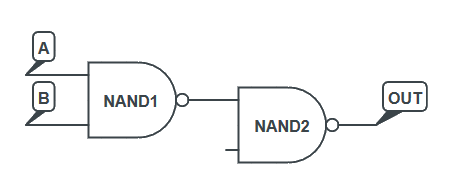
\includegraphics[width=\textwidth]{../grafici/AND1.png}
	\end{minipage}
	\begin{minipage}{0.49\textwidth}
		\centering
		\includegraphics[width=\textwidth]{../grafici/ANDard.pdf}
	\end{minipage}
	\caption{Schema del circuito AND e visualizzazione segnali in I/O}
	\label{fig:AND}
\end{figure}

\paragraph{OR} Si è realizzato il circuito OR con 3 porte NAND.

\begin{figure}[H]
	\centering
	\begin{minipage}{0.49\textwidth}
		\centering
		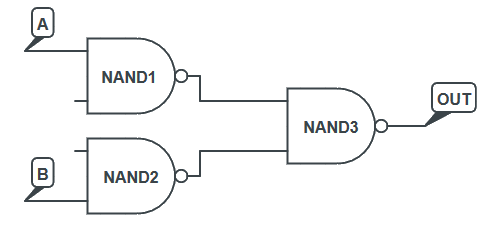
\includegraphics[width=\textwidth]{../grafici/OR1.png}
	\end{minipage}
	\begin{minipage}{0.49\textwidth}
		\centering
		\includegraphics[width=\textwidth]{../grafici/ORard.pdf}
	\end{minipage}
	\caption{Schema del circuito OR e visualizzazione segnali in I/O}
	\label{fig:OR}
\end{figure}

\paragraph{XOR} Si è realizzato il circuito XOR con 4 porte NAND.

\begin{figure}[H]
	\centering
	\begin{minipage}{0.49\textwidth}
		\centering
		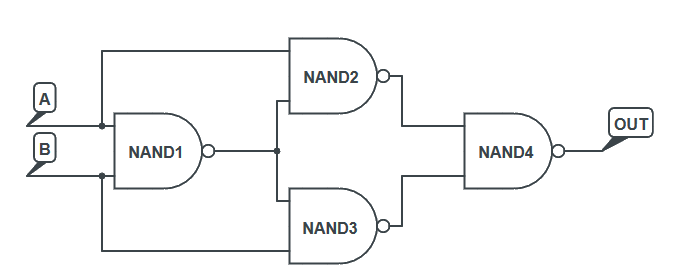
\includegraphics[width=\textwidth]{../grafici/XOR1.png}
	\end{minipage}
	\begin{minipage}{0.49\textwidth}
		\centering
		\includegraphics[width=\textwidth]{../grafici/XORard.pdf}
	\end{minipage}
	\caption{Schema del circuito XOR e visualizzazione segnali in I/O}
	\label{fig:XOR}
\end{figure}


\paragraph{Sommatore ad un bit} Si è realizzato il sommatore ad un bit con 5 porte NAND.

\begin{figure}[H]
	\centering
	\begin{minipage}{0.49\textwidth}
		\centering
		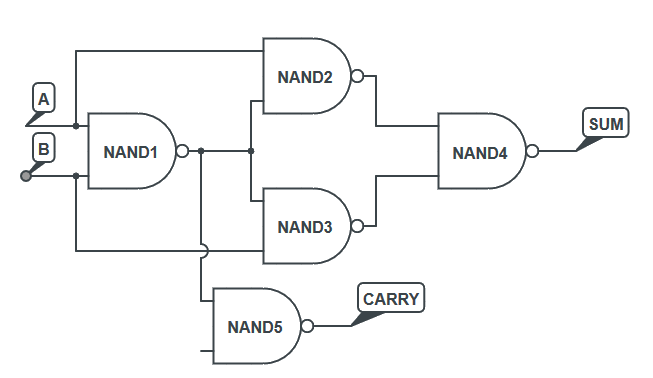
\includegraphics[width=\textwidth]{../grafici/Sommatore1.png}
	\end{minipage}
	\begin{minipage}{0.49\textwidth}
		\centering
		\includegraphics[width=\textwidth]{../grafici/ADDERard.pdf}
	\end{minipage}
	\caption{Schema del sommatore ad un bit e visualizzazione segnali in I/O}
	\label{fig:ADDER}
\end{figure}


\subsection{Osservazione} 

Negli schemi elettrici mostrati nelle \cref{fig:AND,fig:OR,fig:XOR,fig:ADDER} si può notare che per alcune porte NAND si è lasciato un ingresso flottante, quando si voleva usarle come porte NOT. Si è sfruttato infatti il fatto che gli ingressi flottanti delle porte corrispondono ad un valore \code{HIGH}, secondo la logica TTL.
Tenendo conto di questo si ottiene infatti (\code{HIGH-HIGH} $\rightarrow$ \code{LOW}) e (\code{LOW-HIGH} $\rightarrow$ \code{HIGH}), cioè il comportamento richiesto per una porta NOT.

Si sarebbe potuto connettere gli ingressi insieme, così da avere in uscita ancora una volta un NOT, infatti (\code{HIGH-HIGH} $\rightarrow$ \code{LOW}) e (\code{LOW-LOW} $\rightarrow$ \code{HIGH}) secondo la tabella di verità di una porta NAND, ed essere indipendenti dalla logica usata; si è preferito fare così solo per risparmiare qualche connessione sulla basetta e avere un po' più di ordine (fisico, e quindi anche concettuale).

Si è applicato lo stesso metodo anche nei circuito successivi, anche se gli schemi dei circuiti mostrano gli input connessi insieme perché tratti dalla scheda (vedi \cref{fig:MONO,fig:AST,fig:SQGEN}).


\section{Multivibratore MONOSTABILE}
Si è montato il circuito mostrato in \cref{fig:MONO} che rappresenta un Multivibratore Monostabile. 


\begin{figure}[H]
	\centering
	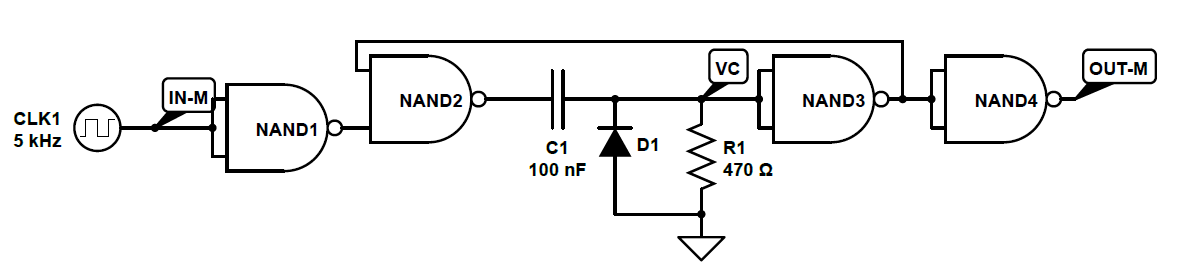
\includegraphics[width=0.9\textwidth]{../grafici/Monostabile.png}
	\caption{Schema del circuito del multivibratore monostabile}
	\label{fig:MONO}
\end{figure}


Si è collegato l'ingresso del multivibratore al generatore di onde, in particolare si è inviata un'onda quadra al suo ingresso con un'ampiezza compresa tra ($88\pm5$)mV e ($4.6\pm0.2$)V , regolando il periodo dell'onda a $(200\pm 1) \mu s$, ossia ad una frequenza di (5000$\pm$25) Hz e il duty cycle (tempo in cui l'onda era a tensione alta rispetto al periodo complessivo) al ($6.7\pm0.3$)\%,. In altre parole si è utilizzato un impulso di $(13.4\pm0.4) \mu s$ ripetuto ogni $(200\pm1) \mu s$.

I componenti impiegati sono stati misurati con il tester digitale, e sono:

\begin{table}[H]
	\centering
	\begin{tabular}{cc}
		$R_1 = \unit{475 \pm5}{\ohm}$ & $C_1 = \unit{108 \pm 5}{\nano\farad}$\\
	\end{tabular}
\end{table}




\paragraph{Funzionamento del circuito}
Si analizzano i grafici mostrati in \cref{fig:OSC,fig:VC} che mostrano rispettivamente le forme d'onda (a regime) in IN-M e OUT-M e le forme d'onda in IN-M e VC, come definiti in \cref{fig:MONO}.

\begin{figure}[H]
	\centering
	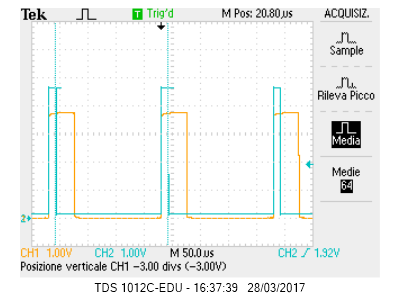
\includegraphics[width=0.58\textwidth]{../grafici/monostabileOSC.png}
	\caption{Forme d'onda visualizzate tramite l'oscilloscopio in ingresso (azzurra) e in uscita (gialla) al multivibratore monostabile.}
	\label{fig:OSC}
\end{figure}

Quando l'onda quadra in ingresso è a $\sim 0V$ (\code{LOW}), all'uscita del NAND1 si è nello stato \code{HIGH}. Supponendo che in partenza  all'uscita del circuito si abbia lo stato \code{LOW}, quindi all'uscita del NAND3 lo stato \code{HIGH}, si ottiene che l'uscita del NAND2 è \code{LOW}\footnote{Lo stato del circuito non sarebbe altrimenti stabile, come descritto sotto, e si transirebbe verso lo stato qui descritto.}. Il condensatore, inizialmente scarico, non si carica e all'ingresso del NAND3 si ha lo stato \code{LOW-LOW}. In questa situazione, finché in ingresso si è nello stato \code{LOW}, il circuito è stabile.

A questo punto l'ingresso passa a \code{HIGH}, quindi l'uscita del NAND2 è \code{HIGH}. Il condensatore inizia a caricarsi attraverso la resistenza $R_1$ e quindi in VC si vede prima il passaggio ad un potenziale\footnote{La carica di un condensatore non è istantanea, quindi quando il NAND2 passa a \code{HIGH},inizialmente entrambe le armature sono ancora allo stesso potenziale, cioè alto.} $V_{max} = 2.93\pm 0.02 V$, e poi la carica di esso, che si manifesta attraverso una discesa esponenziale poiché l'armatura di destra del condensatore si deve caricare negativamente (\cref{fig:VC}).

\begin{figure}[H]
	\centering
	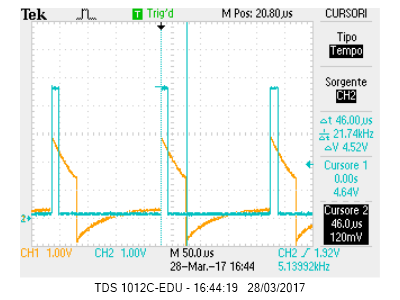
\includegraphics[width=0.6\textwidth]{../grafici/monostabileVC.png}
	\caption{Forme d'onda visualizzate tramite l'oscilloscopio in ingresso (azzurra) e in VC (vedi \cref{fig:MONO}) del multivibratore monostabile.}
	\label{fig:VC}
\end{figure}

Adesso l'ingresso non gioca più alcun ruolo: finché la tensione VC non scende al di sotto di $V_{IH}$ del NAND3, si vedrà la discesa esponenziale dovuta alla carica del condensatore, e quindi la durata dell'impulso (\code{HIGH}) in OUT-M dipende solamente da questa carica, cioè è proporzionale al tempo caratteristico di carica del condensatore $\tau = R_1 C_1 = 51 \pm 3 \mu s$, (la costante di proporzionalità trovata vale 0.87 $\pm$ 0.08) e non dipende dalla durata dell'impulso in IN-M. Questa cosa si è anche verificata modificando l'impulso in IN-M. Il valore di tensione per cui il NAND3 commuta è $V_{com} = 1.44\pm 0.04 V$.

Quando il NAND3 commuta (passa da \code{HIGH-HIGH} a \code{LOW-LOW} al suo ingresso, e quindi in uscita a \code{HIGH}), in seguito al valore scelto per il duty cycle in ingresso al circuito, all'ingresso del NAND1 si è nello stato \code{LOW}, quindi l'uscita del NAND2 è \code{LOW}. In OUT-M il segnale passa quindi da \code{HIGH} a \code{LOW}. Il diodo entra in conduzione (resistenza trascurabile) e l'armatura di destra del condensatore non passa da (\code{HIGH} $-~exp(t/\tau)$) a (\code{LOW} $-~exp(t/\tau)$), ma direttamente ad un valore di potenziale più elevato per cui il diodo non è più in conduzione, il tutto in tempi non apprezzabili sulla scala scelta visualizzata sull'oscilloscopio in \cref{fig:VC}. Il valore del minimo del potenziale\footnote{Tutte le misure dei valori per cui il NAND3 commuta, dei massimi e dei minimi dei potenziali visualizzati in VC, sono calcolate facendo il valor medio e la deviazione standard tra le tre misure trovate analizzando la forma d'onda in \cref{fig:VC}.} è $V_{min} = -0.88\pm 0.04 V$.
% non so che valore guardare sul datasheet, ma ce ne possiamo anche fregare

A questo punto il diodo esce dal regime di conduzione e passa a interdizione; in questo passaggio il condensatore si carica attraverso la resistenza $R_1$ passando da un valore negativo di tensione fino ad una tensione di $\sim 0V$. Quindi alla fine il condensatore risulta scarico e si è tornati nella situazione stabile. Non appena in ingresso al circuito si passa da \code{LOW} a \code{HIGH} il ciclo ricomincia.

La funzione del diodo è quindi di non permettere al potenziale in ingresso del NAND3 di essere troppo negativo, evitando così il malfunzionamento di tale porta.


\subsection{Linearità dell'impulso in uscita al circuito}
Si è verificato che l'andamento dell'impulso in OUT-M in funzione della resistenza $R_1$ fosse lineare, come atteso in seguito alle osservazioni precedenti.
Si sono provati altri $4$ valori per la resistenza $R_1$, oltre a quello impiegato già precedentemente, e si è eseguito un fit lineare con tutti e $5$ i valori. Si riportano dunque il grafico del fit e la tabella con le misure, rispettivamente \cref{fig:MONOfit,tab:MONOfit}.

\begin{figure}[H]
	\centering
	\begin{minipage}{0.49\textwidth}
		\centering
		\includegraphics[width=\textwidth]{../grafici/FITmonostabile.pdf}
		\caption{Grafico dell'impulso in OUT-M in funzione della resistenza $R_1$}
		\label{fig:MONOfit}
	\end{minipage}
	\begin{minipage}{0.49\textwidth}
		\centering
		\resizebox{0.7\textwidth}{!}{
			\input{../tabelle/tab_monostabileRes.txt}}
		\captionof{table}{Resistenze utilizzate per verificare la linearità dell'impulso in OUT-M in funzione della resistenza $R_2$.}
		\label{tab:MONOfit}
	\end{minipage}
\end{figure}

Si riportano di seguito i parametri di fit:

\begin{table}[H]
	\centering
	\begin{tabular}{cccc}
		$\chi^2/ndof = 0.64/3$ & $m = \unit{ 0.110\pm0.006 }{\micro\second / \Omega}$ & $q = \unit{ 7\pm3 }{\micro\second}$ & $corr_{mq} = -0.97 $\\
	\end{tabular}
\end{table}

Dove si è indicato con $m$ il coefficiente angolare, con $q$ l'intercetta e con $corr_{mq}$ il coefficiente di correlazione, che risulta prossimo a ~$-1$ come atteso per una retta. I risultati del fit sono in ottimo accordo con quanto atteso.
% l'errore sui tempi è piccolo perchè mme prende solo la tacca dell'oscilloscopio che è palesemente una sottostima. Ci ho aggiunto il 3% di incertezza sistematica sui tempi, ed esce quello che c'è scritto in tabella tranne il chi2 che esce 18. Cosa metto?

\pagebreak[2]
\section{Multivibratore ASTABILE}

Si è montato il circuito in \cref{fig:AST}.

\begin{figure}[H]
	\centering
	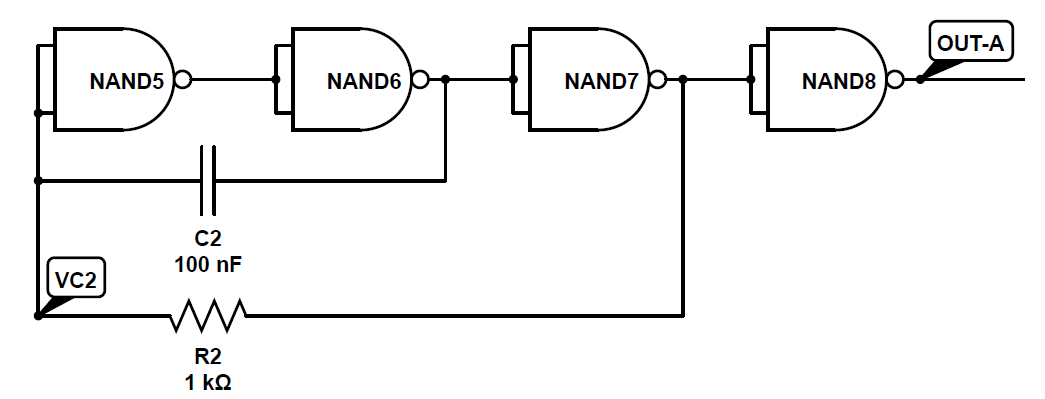
\includegraphics[width=0.7\textwidth]{../grafici/Astabile.png}
	\caption{Schema del circuito del multivibratore astabile}
	\label{fig:AST}
\end{figure}

I componenti impiegati sono stati misurati con il tester digitale, e sono:

\begin{table}[H]
	\centering
	\begin{tabular}{cc}
		$R_2 = \unit{990 \pm 10}{\ohm}$ & $C_2 = \unit{109 \pm 5}{\nano\farad}$\\
	\end{tabular}
\end{table}

Si è verificato che in uscita, OUT-A, la forma d'onda fosse un'onda quadra; si sono misurati il periodo, $\Delta T$, e il duty-cycle, $\delta$, dell'onda, ottenendo:

\begin{table}[H]
	\centering
	\begin{tabular}{cc}
		$\Delta T = \unit{210 \pm 1}{\micro\second}$ (4760$\pm$25 Hz) & $\delta = \unit{72 \pm 4}{\micro\second}$ (34$\pm$2\%)\\
	\end{tabular}
\end{table}

Si riporta quindi la forma d'onda su OUT-A (azzurra) in \cref{fig:ASTosc}, assieme alla forma d'onda presente su VC$2$ (gialla).

\begin{figure}[H]
	\centering
	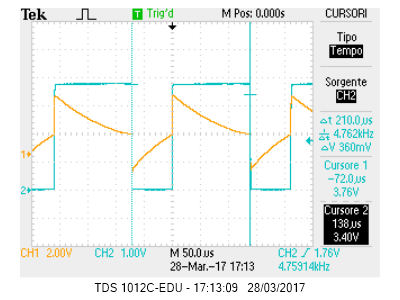
\includegraphics[width=0.7\textwidth]{../grafici/astabileOSC.png}
	\caption{Forme d'onda visualizzate tramite l'oscilloscopio nei punti OUT-A  (azzurra) e VC2 (gialla) della \cref{fig:AST}}
	\label{fig:ASTosc}
\end{figure}

La forma d'onda presente su VC$2$ è il risultato delle curve esponenziali di carica e scarica del condensatore (in realtà sono sempre cariche, perché non si scarica mai liberamente senza una tensione esterna ai capi).

\paragraph{Interpretazione} Per spiegare il comportamento del circuito si deve considerare che la porta NAND$7$ forza la sua uscita ad assumere un valore che sia ben definito, come \code{HIGH} o come \code{LOW}, e altrettanto fa la porta NAND$6$: in questo modo il ramo $R_2-C_2$ ha sempre una differenza di potenziale approssimativamente fissata ai suoi capi, di cui l'unica cosa che varia sostanzialmente è il segno.

Il condensatore si carica dunque, modificando in modo continuo il valore di tensione sul NAND$5$, e raggiunta una data soglia (che risulta essere la stessa in salita in discesa, vedi \cref{fig:ASTosc}), fa commutare NAND5, che a cascata porta tutti gli altri NAND a commutare (sono collegati a catena, l'input di uno all'output del precedente, vedi \cref{fig:AST}).

Il tempo di carica del condensatore è determinato dai valori di $R_2$ e $C_2$, e dalla soglia a cui commuta NAND$5$\footnote{per tempi troppo brevi diventano rilevanti i ritardi delle porte, ma a quel punto non è più possibile considerare come simultanea la commutazione complessiva descritta prima e il circuito può smettere di comportarsi come atteso nel caso descritto}.

Si nota inoltre che all'istante in cui tutte le porte NAND commutano, anche la tensione su VC$2$ salta: infatti il condensatore, che non ha il tempo di scaricarsi, genera la stessa differenza di potenziale tra l'output del NAND$6$ e l'input del NAND$5$ (cioè VC$2$) che generava prima della commutazione, cambiando però istantaneamente il valore dell'output del NAND$6$ cambia pure istantaneamente il valore di VC$2$.

\subsection{Linearità del periodo}
Si è quindi verificato che l'andamento del periodo in funzione della resistenza $R_2$ fosse lineare, come atteso: infatti l'andamento del tempo caratteristico del ramo $R_2-C_2$ è lineare nel valore di $R_2$, ed il periodo è determinato linearmente da tale tempo caratteristico (se il condensatore impiega il doppio del tempo per raggiungere la soglia il periodo sarà doppio).

Si sono provati altri $4$ valori per la resistenza $R_2$, oltre a quello impiegato già precedentemente, e si è eseguito un fit lineare con tutti e $5$ i valori. Si riportano dunque il grafico del fit e la tabella con le misure, rispettivamente \cref{fig:ASTfit,tab:ASTfit}.

\begin{figure}[H]
	\centering
	\begin{minipage}{0.49\textwidth}
		\centering
		\includegraphics[width=\textwidth]{../grafici/FITastabile.pdf}
		\caption{Grafico del periodo in funzione della resistenza $R_2$}
		\label{fig:ASTfit}
	\end{minipage}
	\begin{minipage}{0.49\textwidth}
		\centering
		\resizebox{0.7\textwidth}{!}{
			\input{../tabelle/tab_astabileRes.txt}}
		\captionof{table}{Resistenze utilizzate per verificare la linearità del periodo in funzione di $R_2$.}
		\label{tab:ASTfit}
	\end{minipage}
\end{figure}

Si verifica che la linearità è ottima, e si riportano di seguito i parametri di fit:

\begin{table}[H]
	\centering
	\begin{tabular}{cccc}
		$\chi^2/ndof = 1.60/3$ & $m = \unit{196 \pm 4}{\micro\second / \kilo\ohm}$ & $q = \unit{16 \pm 4}{\micro\second}$ & $corr_{mq} = -0.97$\\
	\end{tabular}
\end{table}

Dove si è indicato con $m$ il coefficiente angolare, con $q$ l'intercetta e con $corr_{mq}$ il coefficiente di correlazione, che risulta prossimo a ~$-1$ come atteso per una retta.

\section{Generatore di onda quadra}

\begin{figure}[H]
	\centering
	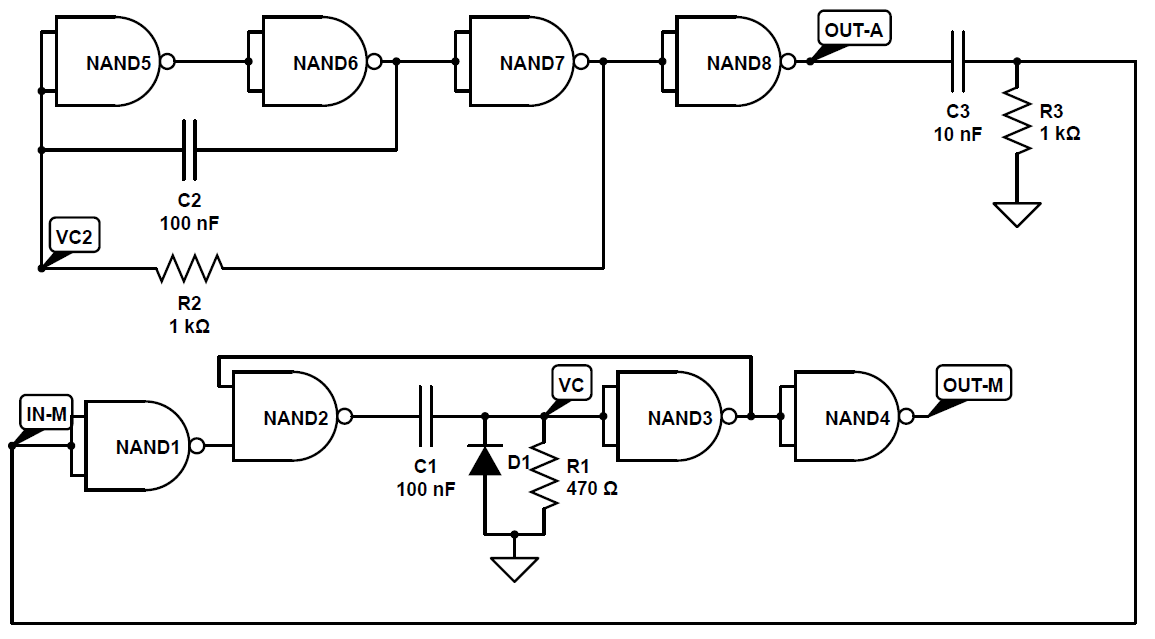
\includegraphics[width=0.8\textwidth]{../grafici/SqGen.png}
	\caption{Schema del circuito del generatore di onda quadra}
	\label{fig:SQGEN}
\end{figure}

\subsection{Forma d'onda in uscita dal derivatore}

Si è dunque messo in serie i due circuiti, collegandoli attraverso un filtro passa-alto (un derivatore) con frequenza di taglio $1/\tau=1/RC=\unit{97 \pm 4}{\kilo\hertz}$
Si è dunque osservato l'output della sezione di alimentazione, a valle del derivatore, e l'output del intero circuito. Come è ben visibile dal oscilloscopio \cref{fig:InMOutM} il multivibratore monostabile è triggerato solo dal fronte d'onda positivo. 

\begin{figure}[H]
	\centering
	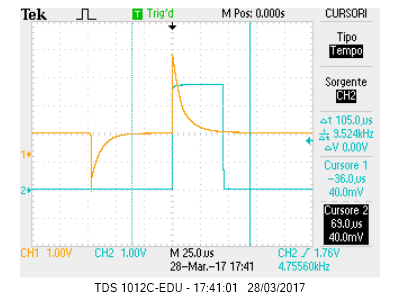
\includegraphics[width=0.8\textwidth]{../grafici/4InMOutM.png}
	\caption{In blu l'output del multistabile (OUT-M), in arancione l'output del derivatore (IN-M)}
	\label{fig:InMOutM}
\end{figure}

\pagebreak[1]
\subsection{Forma d'onda all'uscita complessiva (OUT-M)}

Si è dunque proceduto con la verifica della dipendenza dei due tempi caratteristici del circuito, il periodo e il duty-cycle, dalle resistenze $R_2$ e $R_1$ rispettivamente. Per prima cosa si è fittato, per diversi valori della resistenza $R_2$, la dipendenza del duty-cycle da $R_1$ aspettandoci una dipendenza lineare (in effetti si è svolto un fit affine $t_{duty}=mR_1+q$, anche se di fatto ci si aspetta una dipendenza lineare). I risultati di tali fit sono riassunti in \cref{tab:DutyFit} e nel \cref{fig:FitsRighe}. 

\begin{table}[H]
\centering
\begin{tabular}{c|c|c|c} 
$R_2$ & $T/R$ & $T_0$ & $\chi^2$\\
\hline
673+/-6 & (9.15+/-0.22)e-08 & (-1.9+/-1.3)e-06 & 3.9\\
986+/-9 & (1.102+/-0.029)e-07 & (-8.2+/-1.6)e-06 & 0.518948675843\\
1459+/-13 & (1.212+/-0.023)e-07 & (-1.16+/-0.13)e-05 & 0.990073979354\\
820+/-8 & (1.005+/-0.023)e-07 & (-4.4+/-1.3)e-06 & 1.42818643938\\
1174+/-10 & (1.150+/-0.022)e-07 & (-1.11+/-0.13)e-05 & 2.13024874798\\
\end{tabular}
\caption{Diversi fit del duty-cicle in funzione della resistenza $R_1$ per diversi valori di $R_2$}
\label{tab:DutyFit}
\end{table}

\begin{figure}[H]
	\centering
	\includegraphics[width=0.8\textwidth]{../grafici/FitsRighe.pdf}
	\caption{Diversi fit del duty-cycle in funzione della resistenza $R_1$ per diversi valori di $R_2$}
	\label{fig:FitsRighe}
\end{figure}

Si sono poi presi i diversi valori dei coefficienti angolari $m$ e se ne è trovata la media e la deviazione standard:

\marginpar{\small{Che roba sono i due chiquadri?}}

\begin{table}[H]
\centering
\begin{tabular}{c|c} 
%qunatità & valore\\
%\hline
$m$&$\unit{0.1076 \pm 0.0010}{\micro\second/\ohm}$ \\
$q$&$\unit{-7.4 \pm 0.6}{\micro\second}$ \\
$\chi^2_m$&$109.3$\\
$\chi^2_q$&$41.3$\\
$dof$&$3$\\
\end{tabular}
\end{table}

Si sono anche plottati residui degli scarti in \cref{fig:FitRighe}. \`E chiaramente visibile un andamento sistematico, che con il $\chi^2$ \underline{improbabile} mostrato sopra mostra che il duty-cycle è \underline{solamente approssimativamente}.


\begin{figure}[H]
	\centering
	\includegraphics[width=0.8\textwidth]{../grafici/FitRighe.pdf}
	\caption{Scarti normalizzati di m dalla media e scarti normalizzati di q dalla media}
	\label{fig:FitRighe}
\end{figure}




Si è svolta la stessa procedura per verificare la linearità del periodo rispetto a $R_2$ e la sua indipendenza da $R_1$. Sono stati effettuati i con diversi valori di $R_1$ e sono stati riassunti in \cref{tab:FitsColonne} e nel \cref{fig:FitsColonne}.

\begin{table}[H]
\centering
\begin{tabular}{c|c|c|c} 
$R_1$ & $T/R$ & $T_0$ & $\chi^2$\\
\hline
386+/-4 & (1.973+/-0.035)e-07 & (1.55+/-0.34)e-05 & 0.490688242873\\
820+/-8 & (1.99+/-0.07)e-07 & (1.4+/-0.8)e-05 & 0.234338459765\\
327+/-4 & (1.973+/-0.035)e-07 & (1.55+/-0.34)e-05 & 0.490688242873\\
986+/-9 & (1.97+/-0.04)e-07 & (1.55+/-0.34)e-05 & 0.49060691303\\
475+/-5 & (1.96+/-0.05)e-07 & (1.7+/-0.5)e-05 & 0.338405660518\\
674+/-6 & (1.96+/-0.05)e-07 & (1.6+/-0.5)e-05 & 0.0935217261963\\
558+/-5 & (1.973+/-0.035)e-07 & (1.55+/-0.34)e-05 & 0.490688242873\\
\end{tabular}
\label{tab:FitsColonne}
\end{table}

\begin{figure}[H]
	\centering
	\includegraphics[width=0.8\textwidth]{../grafici/FitsColonne.pdf}
	\caption{Diversi fit del duty-cycle in funzione della resistenza $R_1$ per diversi valori di $R_2$}
	\label{fig:FitsColonne}
\end{figure}


Questa volta $m$ e $q$ sono molto più indipendenti dalla resistenza, cioè più vicino a quanto atteso.

\begin{table}[H]
\centering
\begin{tabular}{c|c} 
%qunatità & valore\\
%\hline
$m$ & $\unit{0.1971 \pm 0.0016}{\micro\second/\ohm} $\\
$q$ & ${15.6 \pm 1.5}{\micro\second}$\\
$\chi^2_m$ & $0.15$\\
$\chi^2_q$ & $0.12$\\
$dof$ & $7$\\
\end{tabular}
\end{table}



Il valore dei $\chi^2$ mostra che gli errori mostrati in \cref{tab:FitsColonne} sono probabilmente sovrastimati. Comunque si può concludere che il periodo è dato da una retta affine rispetto a $R_2$ e che nulla dipende da $R_1$. \underline{In figura gli scarti normalizzati...}

 
\begin{figure}[H]
	\centering
	\includegraphics[width=0.8\textwidth]{../grafici/FitColonne.pdf}
	\caption{Scarti normalizzati di m dalla media e scarti normalizzati di q dalla media}
	\label{fig:FitColonne}
\end{figure}

\subsection{Modulazione periodo e duty-cycle}

Si è dunque provato a trovare dei valori di resistenze $R_1$ e $R_2$ tali da avere un periodo di circa $\unit{100}{\micro\second}$ e un duty-cycle del 30 \%. Si è ottenuto il risultato voluto con $R_1=\unit{386 \pm 5}{\ohm}$ e  $R_1=\unit{434 \pm 5}{\ohm}$. In \cref{fig:410030} il risultato visto all'oscilloscopio. 


 \begin{figure}[H]
	\centering
	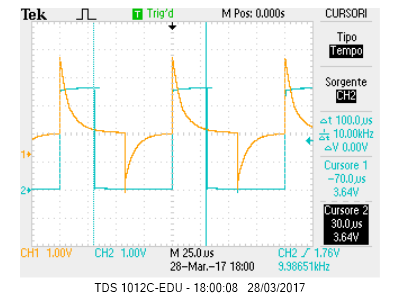
\includegraphics[width=0.8\textwidth]{../grafici/410030.png}
	\caption{In blu l'output del multistabile (OUT-M), in arancione l'output del derivatore (IN-M)}
	\label{fig:410030}
\end{figure}

Come si può vedere dal grafico il periodo è di $\unit{100.0 \pm ?}{\micro\second}$ e il duty-cycle di $\unit{30.0 \pm ?}{\micro\second}$.
\underline{Che bello...}
\marginpar{e gli errori?}



\end{document}